\documentclass[tikz,border=3pt]{standalone}
\usepackage[T1]{fontenc}
\usepackage{times}
\usetikzlibrary{arrows.meta,positioning}
\definecolor{bluea}{HTML}{DCEAF7}
\definecolor{orangea}{HTML}{F9E2CB}
\definecolor{greena}{HTML}{DDEEDC}
\definecolor{graya}{HTML}{ECECEC}
\tikzset{box/.style={draw=black!65,rounded corners=2pt,very thick,align=center,minimum height=12mm,text width=31mm,font=\sffamily\small},arrow/.style={-{Latex[length=2.4mm]},very thick,draw=black!70},note/.style={font=\sffamily\scriptsize,align=center,text=black!75}}
\begin{document}
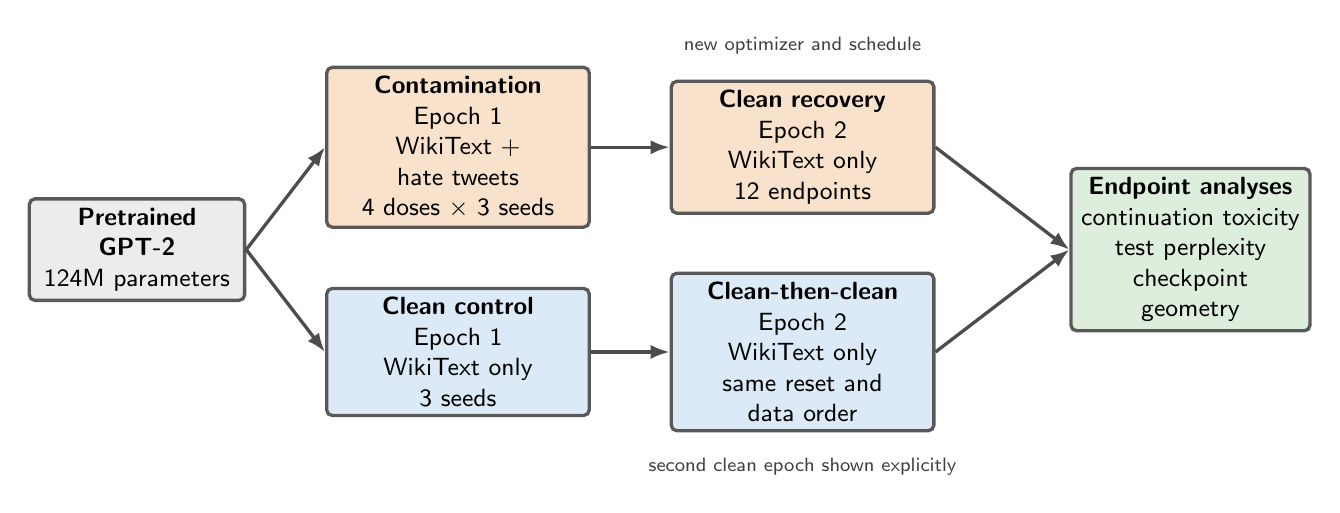
\begin{tikzpicture}[node distance=8mm and 10mm]
\node[box,fill=graya,text width=25mm] (base) {\textbf{Pretrained GPT-2}\\124M parameters};
\node[box,fill=orangea,right=of base,yshift=13mm] (cont) {\textbf{Contamination}\\Epoch 1\\WikiText + hate tweets\\4 doses $\times$ 3 seeds};
\node[box,fill=orangea,right=of cont] (rec) {\textbf{Clean recovery}\\Epoch 2\\WikiText only\\12 endpoints};
\node[box,fill=bluea,right=of base,yshift=-13mm] (clean1) {\textbf{Clean control}\\Epoch 1\\WikiText only\\3 seeds};
\node[box,fill=bluea,right=of clean1] (clean2) {\textbf{Clean-then-clean}\\Epoch 2\\WikiText only\\same reset and data order};
\node[box,fill=greena,right=17mm of rec,yshift=-13mm,text width=28mm] (eval) {\textbf{Endpoint analyses}\\continuation toxicity\\test perplexity\\checkpoint geometry};
\draw[arrow] (base.east) -- (cont.west);
\draw[arrow] (base.east) -- (clean1.west);
\draw[arrow] (cont.east) -- (rec.west);
\draw[arrow] (clean1.east) -- (clean2.west);
\draw[arrow] (rec.east) -- (eval.west);
\draw[arrow] (clean2.east) -- (eval.west);
\node[note,above=2mm of rec] {new optimizer and schedule};
\node[note,below=2mm of clean2] {second clean epoch shown explicitly};
\end{tikzpicture}
\end{document}
